\documentclass[aspectratio=169]{beamer}  
\usefonttheme{professionalfonts}
\usepackage{xeCJK}
\usepackage{fontspec}
\usepackage{graphicx}
\usepackage{listings}
\usepackage{xcolor}
\usepackage{indentfirst}
\usepackage{tikz}
\usepackage{amssymb}
\usepackage{amsthm}
\usepackage{amsmath}
\usepackage{tabularx}
\usepackage{hyperref}
\usepackage{comment}
\usepackage{ulem}
\usepackage{version}
\usepackage{thmtools}
\usepackage{qtree}
\usepackage{algpseudocode}
\usepackage{mathtools}
\usepackage{multicol}
\usepackage{diagbox}

\usefonttheme[onlymath]{serif}

\XeTeXlinebreaklocale "zh"
\XeTeXlinebreakskip = 0pt plus 1pt

\setsansfont{JetBrainsMono-Medium.ttf}
\setCJKmainfont[AutoFakeBold,AutoFakeSlant]{NotoSansTC-Regular.otf}
\usetikzlibrary{arrows,decorations.markings,decorations.pathreplacing}
\newenvironment{Hint}{\noindent\textbf{Hint.}}{}

\tikzstyle {graph node} = [circle, draw, minimum width=1cm]
\tikzset{edge/.style = {decoration={markings,mark=at position 1 with %
            {\arrow[scale=2,>=stealth]{>}}},postaction={decorate}}}

\lstset{
    language=C++,
    basicstyle=\ttfamily\tiny,
    commentstyle=\color{black!50},
    keywordstyle=\color{white!0!blue},
    stringstyle=\color{black!50!green},
    showspaces=false,
    showstringspaces=false,
    showtabs=false,
    tabsize=4,
    captionpos=b,
    breaklines=true,
    breakatwhitespace=false,
    escapeinside={\%*}{*)},
    morekeywords={*}
}

\AtBeginSection[]{
  \begin{frame}
  \vfill
  \centering
  \begin{beamercolorbox}[sep=8pt,center,shadow=true,rounded=true]{title}
    \usebeamerfont{title}\insertsectionhead\par%
  \end{beamercolorbox}
  \vfill
  \end{frame}
}

\title{DP I}
\author{zhu \& sam571128}
\date[附中延平競程讀書會]

\usetheme{Madrid}
\usecolortheme{default}
\setbeamertemplate{itemize items}[square]
\setbeamertemplate{enumerate items}[default]
\setbeamertemplate{blocks}[default]

\begin{document}

    % title
    \begin{frame}
        \titlepage
    \end{frame}

    % contents
    \begin{frame}{這堂課會教的東東 owo}
        \begin{itemize}
            \item 什麼是 DP
            \item 常見 DP 經典題
            \item 背包問題
            \item 其他練習題
        \end{itemize}
    \end{frame}

    % Warm up!
    \begin{frame}[fragile]{Warm up!}
        \begin{block}{\href{https://leetcode.com/problems/climbing-stairs/}{走樓梯}}
            有一個 $n$ 階的樓梯,每次可以走一格或是兩格,求走到第 $n$ 階有幾種走法?
        \end{block}
        \begin{itemize}
            \item<2-> 學過遞迴的應該都會知道要怎麼做了 >< \pause
            \item<3-> 令 $F(n)$ 為走到第 $n$ 階的方法數 \pause
            \item<3-> 有兩種可能,一種是從 $n-1$ 階走一步過來,另一種是從 $n-2$ 階走兩步過來 \pause
            \item<4-> 那遞迴式就是 $F(n) = F(n-1) + F(n-2)$ \pause
            \item<5-> 且遞迴終止條件為 $F(0) = 1, F(1) = 1$ \pause
        \end{itemize} 
        \begin{lstlisting}[language=C++, basicstyle= \ttfamily \small]
  int F(int n){
      if(n<=1) return 1;
      else return (F(n-1)+F(n-2));
  }
        \end{lstlisting}
    \end{frame}
    \begin{frame}{Warm up!}
        \begin{itemize}
            \item 你會發現吃 TLE 了
            \item<2-> why?
            \item<3-> 在自己的電腦跑一次,你會發現當 $n = 50$ 的時候就很慢了
            \item<4-> 複雜度大約是 $O(F(n))$,那其實這是一個指數級成長的函數
        \end{itemize}
    \end{frame}
    
    \begin{frame}{Warm up!}
        \begin{itemize}
            \item 觀察下圖,我們可以發現有很多狀態會被重複使用到
            \item<2-> 用前面的暴力遞迴,這些狀態每次都要重複算
        \end{itemize}
        \begin{center}
            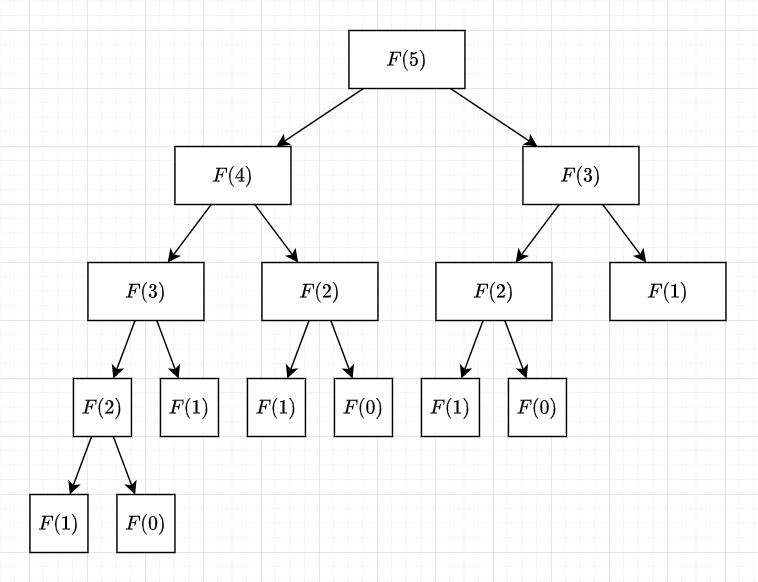
\includegraphics[scale=0.35]{images/fibonacci_tree.png}
        \end{center}
    \end{frame}
    
    \begin{frame}{Warm up!}
        \begin{itemize}
            \item 我們可以多開一個陣列用來記錄已經計算過的狀態!
            \item<2-> 這個動作叫做記憶化 (Memoization)
        \end{itemize}
        \begin{center}
            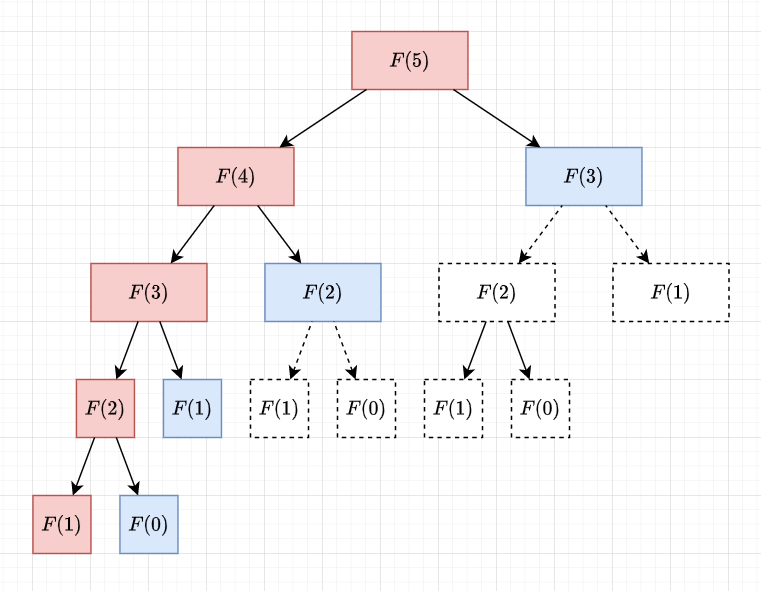
\includegraphics[scale=0.35]{images/fibonacci_memo.png}
        \end{center}
    \end{frame}

    \begin{frame}[fragile]{Warm up!}
        \begin{itemize}
            \item 將狀態記錄下來後,複雜度從指數級變成線性 $O(n)$
            \item<2-> 「記憶化」就是動態規劃的基本精神!
        \end{itemize} 
        \begin{lstlisting}[language=C++, basicstyle= \ttfamily \small]
    int F(int n){
        if(n<=1) return 1;
        else if(dp[i]) return dp[i];
        else return (dp[i]=F(i-1)+F(i-2));
    }
        \end{lstlisting}
    \end{frame}
    
    \section{什麼是 DP?}
    
    % start

    % what is dp
    \begin{frame}{甚麼是動態規劃?}
        \begin{itemize}
            \item 動態規劃(Dynamic Programming),簡稱 DP \pause
            \item<2-> 他不是演算法,比較像是一種想法或技巧 \pause
        \end{itemize}
        \vspace{5mm}
        \begin{center}
            
\includegraphics[]{images/dp_name_of_array.png}
        \end{center}
    \end{frame}

    % somthing about dp
    \begin{frame}{一些 DP 的性質}
        \begin{itemize}
            \item 重複子問題 (overlapping subproblems)
            \begin{enumerate}
                \item 同樣性質的子問題,會被重複計算
                \item 可以使用「記憶化」來避免重複計算
            \end{enumerate}
            \item 最佳子結構 (optimal substructures)
            \begin{enumerate}
                \item 對於某個狀態的最佳解,可以從小狀態的最佳解轉移過來
            \end{enumerate}
            \item 無後效性
            \begin{enumerate}
                \item 轉移順序必須是一張 DAG (有向無環圖),子問題之間不會互相呼叫
                \item 因此轉移順序很重要
            \end{enumerate}
        \end{itemize}
    \end{frame}

    % dp step
    \begin{frame}{dp 的步驟 (以走樓梯為例)}
        \begin{alertblock}{step 1 設置狀態}
            一個狀態其實就是一個子問題。令 $dp[i]$ 表示走到第 $i$ 階的方法數
        \end{alertblock}
        
        \setbeamercolor{block title}{use=structure,bg=green!50!black}
        \begin{block}{step 2 導出轉移}
            思考要怎麼從其他以計算過的狀態求解  \\
            \begin{center}
                $dp[i] = dp[i-1] + dp[i-2]$
            \end{center}
        \end{block}
        
        \setbeamercolor{block title}{use=structure,bg=blue!60!black}
        \begin{block}{step 3 打好基底}
            基底可以是遞迴的終止條件或是迴圈中的邊界條件 \\
            \begin{center}
                $dp[0] = 1, \ dp[1] = 1$   
            \end{center}
        \end{block}
    \end{frame}

    % dp implementation
    \begin{frame}{dp 的實作}
        \begin{itemize}
            \item Top-down
            \begin{enumerate}
                \item 從大子問題去找小子問題
                \item 實作方式通常是遞迴
                \item 轉移式列出來其實就差不多了
                \item 需要遞迴終止條件

            \end{enumerate}
            \item Buttom-up
            \begin{enumerate}
                \item 從小子問題去推到大子問題
                \item 實作方式是用迴圈
                \item 比較需要去注意轉移順序
                \item 需要初始化邊界條件
            \end{enumerate}
            \item 我個人比較習慣都寫迴圈,所以之後放的程式碼大部分都會是迴圈版的 ><
        \end{itemize}
    \end{frame}

    % classic problems
    \section{常見 DP 經典題}

    \begin{frame}{常見 DP 經典題}
        \begin{itemize}
            \item 接下來每題大概給 3~5 分鐘的思考時間 ><
            \item 按照步驟:設置狀態、導出轉移、打好基底
        \end{itemize}
    \end{frame}

    % 0
    \begin{frame}{常見 DP 經典題 - 0}
        \begin{block}{\href{https://atcoder.jp/contests/dp/tasks/dp_b}{AtCoder DP Contest pB - Frog 2}}
            給你 $N$ 顆石頭,對於每個石頭 $i$,它的高度為 $h_i$。一開始在第 $1$ 個石頭上,每次可以往前跳 $1 \sim K$ 格,從第 $i$ 個石頭跳到第 $j$ 個石頭的花費是 $|h_i - h_j|$,求跳到第 $N$ 格的最小花費 \\
            \vspace{2.5mm}
            \begin{itemize}
                \item $1 \le N \le 10^5$
                \item $1 \le K \le 100$
            \end{itemize}
        \end{block}
    \end{frame}

    \begin{frame}{常見 DP 經典題 - 0}
        \begin{alertblock}{step 1 設置狀態}
            令 $dp[i]$ 為從第 $1$ 顆石頭跳到第 $i$ 顆石頭的最小花費
        \end{alertblock}
    \end{frame}
    \begin{frame}{常見 DP 經典題 - 0}
        \setbeamercolor{block title}{use=structure,bg=green!50!black}
        \begin{block}{step 2 導出轉移}
            枚舉最後一次跳了幾步,假設最後一次跳了 $j$ 步,則轉移式就會是
            $$dp[i] = \min_{j=1}^k(dp[i-j] + |h_i-h_j|)$$
        \end{block}
     \end{frame}  
     \begin{frame}{常見 DP 經典題 - 0}
        \setbeamercolor{block title}{use=structure,bg=blue!60!black}
        \begin{block}{step 3 打好基底}
            在第一顆石頭的時候不會有任何花費,所以有 $dp[1] = 0$
        \end{block}
    \end{frame}
    \begin{frame}[fragile]{常見 DP 經典題 - 0}
        \begin{lstlisting}[language=C++, basicstyle=\ttfamily\tiny]
#include <bits/stdc++.h>
#define fastio ios_base::sync_with_stdio(false);cin.tie(0);

using namespace std;

signed main(){
    fastio

    int n,k;cin>>n>>k;
    int h[n+1]{},dp[n+1]{};
    for(int i=1;i<=n;++i) cin>>h[i];
    for(int i=2;i<=n;++i){
        dp[i]=1e9;
        for(int j=1;j<=k;++j){
            if(i-j>=1) dp[i]=min(dp[i],dp[i-j]+abs(h[i]-h[i-j]));
        }
    }

    cout<<dp[n]<<'\n';
}
        \end{lstlisting}
    \end{frame}

    % 1
    \begin{frame}{常見 DP 經典題 - 1}
        \begin{block}{\href{https://atcoder.jp/contests/dp/tasks/dp_c}{AtCoder DP Contest pC - Vacation}}
            有 $N$ 天的假期,並且有 $a, b, c$ 三種活動 \\
            \begin{enumerate}
                \item 在第 $i$ 天做活動 $a$ 會獲得 $a_i$ 點的快樂值
                \item 在第 $i$ 天做活動 $b$ 會獲得 $b_i$ 點的快樂值
                \item 在第 $i$ 天做活動 $c$ 會獲得 $c_i$ 點的快樂值
            \end{enumerate}
            但為了避免對活動感到厭倦,不可以兩天以上都進行同一種活動 \\
            求 $N$ 天後的最大快樂值
            \vspace{2.5mm}
            \begin{itemize}
                \item $1 \leq n \leq 10^5$
                \item $1 \leq a_i, b_i, c_i \leq 10^4$
            \end{itemize}
        \end{block}
    \end{frame}

    \begin{frame}{常見 DP 經典題 - 1}
        \begin{alertblock}{step 1 設置狀態}
            令 $dp[i]$ 為第 $i$ 天結束後的最大快樂值 \\
            \vspace{2mm}
            那麼答案就會是 $dp[N]$
        \end{alertblock}
        \begin{itemize}
            \item<2-> 好像列不出正確的轉移?
            \item<3-> 沒關係!一維不夠就讓他多一維!
        \end{itemize}
    \end{frame}

    \begin{frame}{常見 DP 經典題 - 1}
        \begin{alertblock}{step 1 設置狀態}
            令 $dp[i][j]$ 為在第 $i$ 天做完第 $j$ 種活動後的最大快樂值($j = 0, 1, 2$) \\
            \vspace{2mm}
            那麼答案就會是 $\max(dp[N][0], \ dp[N][1], \ dp[N][2])$
        \end{alertblock}
    \end{frame}
    \begin{frame}{常見 DP 經典題 - 1}
        \setbeamercolor{block title}{use=structure,bg=green!50!black}
        \begin{block}{step 2 導出轉移}
            題目有條件是「不可以兩天以上都進行同一種活動」,故轉移式為 \\
            $$dp[i][0] = \max(dp[i-1][1], \ dp[i-1][2]) + a_i$$
            $$dp[i][1] = \max(dp[i-1][0], \ dp[i-1][2]) + b_i$$
            $$dp[i][2] = \max(dp[i-1][0], \ dp[i-1][1]) + c_i$$
        \end{block}
    \end{frame}
     \begin{frame}{常見 DP 經典題 - 1}   
        \setbeamercolor{block title}{use=structure,bg=blue!60!black}
        \begin{block}{step 3 打好基底}
            顯然有 $dp[1][0] = a[1], \ dp[1][1] = b[1], \ dp[1][2] = c[1]$
        \end{block}
    \end{frame}

    \begin{frame}[fragile]{常見 DP 經典題 - 1}
        \begin{lstlisting}[language=C++, basicstyle=\ttfamily\tiny]
#include <bits/stdc++.h>
#define fastio ios_base::sync_with_stdio(false);cin.tie(0);

using namespace std;

signed main(){
    fastio

    int n;cin>>n;
    int a[n+1]{},b[n+1]{},c[n+1]{},dp[n+1][3]{};
    for(int i=1;i<=n;++i) cin>>a[i]>>b[i]>>c[i];
    
    dp[1][0]=a[1],dp[1][1]=b[1],dp[1][2]=c[1];
    for(int i=2;i<=n;++i){
        dp[i][0]=max(dp[i-1][1],dp[i-1][2])+a[i];
        dp[i][1]=max(dp[i-1][0],dp[i-1][2])+b[i];
        dp[i][2]=max(dp[i-1][0],dp[i-1][1])+c[i];
    }
    cout<<max({dp[n][0],dp[n][1],dp[n][2]})<<'\n';
}     
        \end{lstlisting}
    \end{frame}
    
    % 2
    \begin{frame}{常見 DP 經典題 - 2}
        \begin{block}{\href{https://cses.fi/problemset/task/1643/}{CSES Maximum Subarray Sum}}
            求連續子陣列最大和(最長連續子陣列:陣列中一段連續的數字)\\
            \vspace{2.5mm}
            \begin{itemize}
                \item $1 \leq n \leq 2 \cdot 10^5$
            \end{itemize}
        \end{block}
    \end{frame}
    
    \begin{frame}{常見 DP 經典題 - 2}
        \begin{alertblock}{step 1 設置狀態}
            令 $dp[i]$ 為前 $i$ 項(包含第 $i$ 項)的連續子陣列最大和 \\
            \vspace{2mm}
            那麼答案就會是 $dp[1] \sim dp[n]$ 的最大值
        \end{alertblock}
    \end{frame}
    \begin{frame}{常見 DP 經典題 - 2}
        \setbeamercolor{block title}{use=structure,bg=green!50!black}
        \begin{block}{step 2 導出轉移}
            對於每個 $i$,可以分成選 $i-1$ 以前的或是不選 $i-1$ 以前的 \\
            $$dp[i] = \max( a[i] + dp[i-1], a[i] )$$
        \end{block}
    \end{frame}
    \begin{frame}{常見 DP 經典題 - 2}
        \setbeamercolor{block title}{use=structure,bg=blue!60!black}
        \begin{block}{step 3 打好基底}
            題目說至少要選取一個數,那顯然有 $dp[1] = a[1]$
        \end{block}
    \end{frame}

    \begin{frame}[fragile]{常見 DP 經典題 - 2}
        \begin{lstlisting}[language=C++, basicstyle=\ttfamily\tiny]
#include <bits/stdc++.h>
#define fastio ios_base::sync_with_stdio(false);cin.tie(0);

using namespace std;

signed main(){
    fastio
 
    int n;cin>>n;
    long long a[n+1]{},dp[n+1]{},mx=-1e18;
    for(int i=1;i<=n;++i) cin>>a[i];
    dp[1]=a[1];
    for(int i=1;i<=n;++i){
        dp[i]=max(dp[i-1]+a[i],a[i]);
        mx=max(mx,dp[i]);
    }
    cout<<mx<<'\n';
}
        \end{lstlisting}
    \end{frame}

    % 3
    \begin{frame}{常見 DP 經典題 - 3}
        \begin{block}{\href{https://zerojudge.tw/ShowProblem?problemid=c001}{ZeroJudge Longest Common Subsequence}}
            給兩個字串 $a, b$,長度為 $n, m$,求他們的最長共同子序列(LCS)\\
            \vspace{2.5mm}
            \begin{itemize}
                \item $1 \leq n, m \leq 1000$
            \end{itemize}
        \end{block}
        \begin{itemize}
            \item<2-> $a = \texttt{abcdgh}$, $b = \texttt{aedfhr}$
            \item<2-> 那他們的 LCS 就是 a, d, h
        \end{itemize}
    \end{frame}

    \begin{frame}{常見 DP 經典題 - 3}
        \begin{alertblock}{step 1 設置狀態}
            令 $dp[i][j]$ 為在字串 $a$ 的前 $i$ 個字母與字串 $b$ 的前 $j$ 個字母的 LCS 長度 \\
            \vspace{2mm}
            那麼答案就會是 $dp[n][m]$
        \end{alertblock}
    \end{frame}
    \begin{frame}{常見 DP 經典題 - 3}
        \setbeamercolor{block title}{use=structure,bg=green!50!black}
        \begin{block}{step 2 導出轉移}
            若 $a[i] = b[j]$,兩字串最後的字母是相同的,所以 $dp[i][j] = dp[i-1][j-1]+1$ \\
            \vspace{2mm}
            否則 $dp[i][j] = \max(dp[i-1][j], dp[i][j-1])$
        \end{block}
    \end{frame}
    \begin{frame}{常見 DP 經典題 - 3}
        \setbeamercolor{block title}{use=structure,bg=blue!60!black}
        \begin{block}{step 3 打好基底}
            如果其中一個字串長度為 $0$,則他們的 LCS 就是 $0$
            $$dp[i][0] = 0, dp[0][j] = 0$$
        \end{block}
    \end{frame}

    \begin{frame}[fragile]{常見 DP 經典題 - 3}
        \begin{lstlisting}[language=C++, basicstyle=\ttfamily\tiny]
#include <bits/stdc++.h>
#define fastio ios_base::sync_with_stdio(false);cin.tie(0);

using namespace std;

signed main(){
    fastio

    string a;
    while(cin>>a){
        string b;cin>>b;
        int alen=a.length(),blen=b.length();
        a=" "+a,b=" "+b;
        int dp[alen+1][blen+1]{};
        for(int i=1;i<=alen;++i){
            for(int j=1;j<=blen;++j){
                if(a[i]==b[j]) dp[i][j]=dp[i-1][j-1]+1;
                else dp[i][j]=max(dp[i-1][j],dp[i][j-1]);
            }
        }
        cout<<dp[alen][blen]<<'\n';
    }
}
        \end{lstlisting}
    \end{frame}
    
    % 4
    \begin{frame}{常見 DP 經典題 - 4}
        \begin{block}{\href{https://cses.fi/problemset/task/1639/}{CSES Edit Distance}}
            給定兩個字串 $a, b$,長度分別為 $n, m$,以下有三種操作: \\
            1. 加一個字母到字串$a$中 \\
            2. 刪除字串$a$中的一個字母 \\
            3. 將字串$a$中的字母替換成你想要的字母 \\
            求最少要幾次操作才使得兩個字串相同 \\
            \vspace{2.5mm}
            \begin{itemize}
                \item $1 \leq n, m \leq 5000$
            \end{itemize}
        \end{block}
    \end{frame}

    \begin{frame}{常見 DP 經典題 - 4}
        \begin{alertblock}{step 1 設置狀態}
            令 $dp[i][j]$ 為在字串 $a$ 取到第 $i$ 個字母且在字串 $b$ 取到第 $j$ 個字母的最少操作數 \\
            \vspace{2mm}
            那麼答案就會是 $dp[n][m]$
        \end{alertblock}
    \end{frame}

    \begin{frame}{常見 DP 經典題 - 4}
        \setbeamercolor{block title}{use=structure,bg=green!50!black}
        \begin{block}{step 2 導出轉移}
            $$
            dp[i][j]= \min
            \begin{cases}
                dp[i-1][j-1]         & \text{if } s[i]=s[j] \\
                dp[i][j-1]+1         & \text{對 a 加上字母 b[i]} \\
                dp[i-1][j]+1         & \text{刪除 a 的最後一個字母 a[i]} \\
                dp[i-1][j-1]+1       & \text{把 a 的最後一個字母換成 b 的最後一個字母} \\
            \end{cases}
            $$
        \end{block}
    \end{frame}

    \begin{frame}{常見 DP 經典題 - 4}
        \setbeamercolor{block title}{use=structure,bg=blue!60!black}
        \begin{block}{step 3 打好基底}
            $$dp[0][0] = 0, \ dp[i][0] = i, \ dp[0][j] = j$$
        \end{block}
    \end{frame}

    \begin{frame}[fragile]{常見 DP 經典題 - 4}
        \begin{lstlisting}[language=C++, basicstyle=\ttfamily\tiny]
#include <bits/stdc++.h>
#define fastio ios_base::sync_with_stdio(false);cin.tie(0);

using namespace std;

signed main(){
    fastio
 
    string a,b;cin>>a>>b;
    int alen=a.length(),blen=b.length();
    a=" "+a,b=" "+b;
    int dp[alen+1][blen+1]{};
    for(int i=1;i<=alen;++i) dp[i][0]=i;
    for(int i=1;i<=blen;++i) dp[0][i]=i;
    for(int i=1;i<=alen;++i){
        for(int j=1;j<=blen;++j){
            if(a[i]==b[j]) dp[i][j]=dp[i-1][j-1];
            else dp[i][j]=min({dp[i-1][j]+1,dp[i][j-1]+1,dp[i-1][j-1]+1});
        }
    }
    cout<<dp[alen][blen]<<'\n';
}
        \end{lstlisting}
    \end{frame}

    % 5
    \begin{frame}{常見 DP 經典題 - 5}
        \begin{block}{\href{https://cses.fi/problemset/task/1638}{CSES Grid Paths}}
            給一個 $n \times n$ 的網格圖,只能往下或往右走,不能走到陷阱,問有幾種走法 \\
            \vspace{2.5mm}
            \begin{itemize}
                \item $1 \leq n \leq 1000$
            \end{itemize}
        \end{block}
    \end{frame}

    \begin{frame}{常見 DP 經典題 - 5}
        \begin{alertblock}{step 1 設置狀態}
            令 $dp[i][j]$ 為走到 $(i, j)$ 的方法數 \\
            \vspace{2mm}
            那麼答案就會是 $dp[n][n]$
        \end{alertblock}
    \end{frame}
    \begin{frame}{常見 DP 經典題 - 5}
        \setbeamercolor{block title}{use=structure,bg=green!50!black}
        \begin{block}{step 2 導出轉移}
            有兩種情況
            $$
            dp[i][j]= 
            \begin{cases}
                0 & \text{若 (i,j) 有陷阱} \\
                dp[i-1][j] + dp[i][j-1]           & \text{Otherwise} \\
            \end{cases}
            $$
        \end{block}
    \end{frame}  
    \begin{frame}{常見 DP 經典題 - 5}
        \setbeamercolor{block title}{use=structure,bg=blue!60!black}
        \begin{block}{step 3 打好基底}
            如果 $(1,1)$ 沒有陷阱,$dp[1][1]=1$,否則 $dp[i][j]$ 皆為 $0$
        \end{block}
    \end{frame}

    \begin{frame}[fragile]{常見 DP 經典題 - 5}
        \begin{lstlisting}[language=C++, basicstyle=\ttfamily\tiny]
#include <bits/stdc++.h>
#define fastio ios_base::sync_with_stdio(0); cin.tie(0);

using namespace std;

const int MOD = 1e9+7;

signed main(){
    fastio

    int n;cin>>n;
    char g[n+1][n+1]{};

    for(int i=1;i<=n;++i){
        for(int j=1;j<=n;++j) cin>>g[i][j];
    }
    
    int dp[n+1][n+1]{};
    for(int i=1;i<=n;++i){
        for(int j=1;j<=n;++j){
            if(g[i][j]=='*') dp[i][j]=0;
            else if(i==1&&j==1) dp[i][j]=1;
            else dp[i][j]=(dp[i-1][j]+dp[i][j-1])%MOD;
        }
    }
    cout<<dp[n][n]%MOD<<'\n';
}
        \end{lstlisting}
    \end{frame}

    % 6
    \begin{frame}{常見 DP 經典題 - 6}
        \begin{block}{\href{https://cses.fi/problemset/task/1145}{CSES Increasing Subsequence}}
            給長度為 $n$ 的序列,求最長遞增子序列(LIS)長度
            \vspace{2.5mm}
            \begin{itemize}
                \item $1 \leq n \leq 2 \cdot 10^5$
            \end{itemize}
        \end{block}
        \begin{itemize}
            \item<2-> $A = \{7,3,5,3,6,2,9,8 \}$
            \item<2-> LIS 長度為 $4$
        \end{itemize}
    \end{frame}

    \begin{frame}{常見 DP 經典問題 - 6}
        \begin{itemize}
            \item 看到 $n$ 的範圍,感覺就是 $O(n)$ 或 $O(n \log n)$ 之類的東西
            \item<2-> 一時間好像想不到複雜度會過的解 ...
            \item<3-> 沒關係!一樣可以先列出 DP 式再去思考要怎麼優化他!
        \end{itemize}
    \end{frame}

    \begin{frame}{常見 DP 經典題 - 6}
        \begin{alertblock}{step 1 設置狀態}
            令 $dp[i]$ 為最後一個數為 $a[i]$ 的最長遞增遞增子序列長度 \\
            \vspace{2mm}
            那麼答案就是 
            $$\max_{j=1}^n(dp[j])$$
        \end{alertblock}
    \end{frame}
    \begin{frame}{常見 DP 經典題 - 6}
        \setbeamercolor{block title}{use=structure,bg=green!50!black}
        \begin{block}{step 2 導出轉移}
            對於所有位置在 $i$ 之前,且小於 $a[j]$ 的數,可以在他後面接上 $a[j]$,長度 $+1$ \\
            $$dp[i] = \max_{j < i, a[j] < a[i]}(dp[j]+1)$$
        \end{block}
    \end{frame}  
    \begin{frame}{常見 DP 經典題 - 6}
        \setbeamercolor{block title}{use=structure,bg=blue!60!black}
        \begin{block}{step 3 打好基底}
            有兩種方式
            \begin{enumerate}
                \item $dp[0]=0$,把 $a[0] := -\infty$,在沒有數字時,LIS 長度為 $0$
                \item $dp[i]=1$,所有結尾在 $a[i]$ 的 LIS 最短長度會是 $1$ (自己一個)
            \end{enumerate}
        \end{block}
    \end{frame}
    
    \begin{frame}[fragile]{常見 DP 經典題 - 6 - $O(n^2)$ }
        \begin{lstlisting}[language=C++, basicstyle=\ttfamily\tiny]
#include <bits/stdc++.h>
#define fastio ios_base::sync_with_stdio(false);cin.tie(0);

using namespace std;
 
signed main(){
    fastio
 
    int n;cin>>n;
    vector<int> a(n+1),dp(n+1,0);
    for(int i=1;i<=n;++i) cin>>a[i];
    for(int i=1;i<=n;++i){
        for(int j=0;j<=i;++j){
            if(a[j]<a[i]) dp[i]=max(dp[i],dp[j]+1);
        }
    }
    cout<<*max_element(dp+1,dp+n+1)<<'\n';
}
        \end{lstlisting}
    \end{frame}
    
    \begin{frame}{常見 DP 經典題 - 6}
        \begin{itemize}
            \item 咦 他的複雜度是 $O(n^2)$ 欸!這樣會 TLE!
            \item<2-> 想想看有哪裡優化?
            \item<3-> 這個技巧沒看過的應該很難想到,所以我會直接講解
        \end{itemize}
    \end{frame}

    \begin{frame}{常見 DP 經典題 - 6}
        \begin{itemize}
            \item 開一個 $v$,而 $v[j]$ 表示對於所有 $dp[i] = j$ 的最小 $a[i]$
            \item 邊二分搜邊更新 $dp[i]$ 和 $v$ 
            \item<2-> 這樣時間複雜度會是 $O(n\log n)$
        \end{itemize}
        \begin{center}
            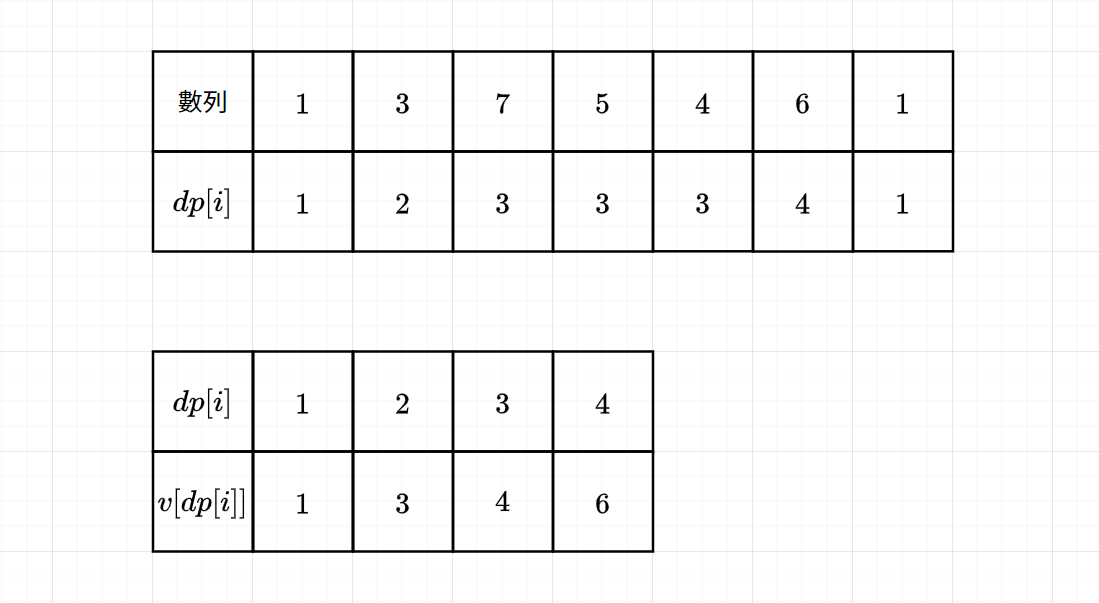
\includegraphics[scale=0.3]{images/LIS_Table.png}
        \end{center}
    \end{frame}
    
    \begin{frame}[fragile]{常見 DP 經典題 - 6 - $O(n \log n)$ }
        \begin{lstlisting}[language=C++, basicstyle=\ttfamily\tiny]
#include <bits/stdc++.h>
#define fastio ios_base::sync_with_stdio(false);cin.tie(0);

using namespace std;
 
signed main(){
    fastio
 
    int n;cin>>n;
    vector<int> a(n+1),v,dp(n+1,0);
    for(int i=0;i<n;++i) cin>>a[i];
    for(int i=0;i<n;++i){
        int num=lower_bound(v.begin(),v.end(),a[i])-v.begin();
        dp[i]=num+1;
        if(num==v.size()) v.emplace_back(a[i]);
        else v[num]=a[i];
    }
    cout<<v.size()<<'\n';
}
        \end{lstlisting}
    \end{frame}

    \section{背包問題}

    \begin{frame}{Warm up!}
        \begin{block}{簡單的硬幣問題}
        給你無限個 1 元、5 元、8 元的硬幣,請問最少需要多少硬幣才能湊出 $x$ 元?
        \end{block} 
        \begin{itemize}
            \item<2-> 還記得之前 greedy 的時候講過的最佳策略嗎?
            \item<3-> 先從幣值大的開始選,如果會超過$x$,就往小的選
            \item<4-> 這樣真的會是最佳解嗎?
        \end{itemize}
    \end{frame}

    \begin{frame}{背包問題 - 0}
        \begin{block}{\href{https://atcoder.jp/contests/dp/tasks/dp_d}{Atcoder DP Contest D - Knapsack 1}}
            有 $N$ 個物品,每個物品有價值 $v_i$ 和大小 $w_i$,每個物品只有一個。你有一個容量為 $W$ 的背包。請問你最多可以拿多少價值?
        \end{block}
        \begin{itemize}
            \item<2-> 這題是經典的 0/1 背包問題
            \item<2-> 其實也就是每個東西只有一個,要嘛選要嘛不選
        \end{itemize}
    \end{frame}

    \begin{frame}{背包問題 - 0}
        \begin{alertblock}{step 1 設置狀態}
            令$dp[i][j]$為取到第$i$個物品且重量為$j$時的最大價值\\
            \vspace{2mm}
            那麼答案就是 $dp[N][W]$
        \end{alertblock}
    \end{frame}

    \begin{frame}{背包問題 - 0}
        \setbeamercolor{block title}{use=structure,bg=green!50!black}
        \begin{block}{step 2 導出轉移}
            對於每個物品,可以選或不選\\
            $$
            dp[i][j]= \max
            \begin{cases}
                dp[i-1][j-w[i]]+v[i] & \text{選物品} \\
                dp[i-1][j]           & \text{不選物品} \\
            \end{cases}
            $$
        \end{block}
    \end{frame}  

    \begin{frame}{背包問題 - 0}
        \setbeamercolor{block title}{use=structure,bg=blue!60!black}
        \begin{block}{step 3 打好基底}
            以這題來講,因為它的價值皆為正,
            當你未選取任何物品(重量為$0$)時,價值為 $0$
            $$dp[0][i] = 0, \ dp[j][0] = 0, \text{for all } i,j$$
        \end{block}
    \end{frame}

    \begin{frame}{背包問題 - 0}
        \begin{itemize}
            \item 觀察一下轉移式
            $$
            dp[i][j]= \max
            \begin{cases}
                dp[i-1][j-w[i]]+v[i] & \text{選物品} \\
                dp[i-1][j]           & \text{不選物品} \\
            \end{cases}
            $$
            \item<2-> 可以發現我們的每個狀態都是從 $i-1$ 轉移過來的
            \item<3-> 轉移後 $i-1$ 那格的狀態已經不重要了
            \item<4-> 所以其實是可以做到一維的!
        \end{itemize}
    \end{frame}
    
    \begin{frame}{背包問題 - 0}
        \begin{center}
            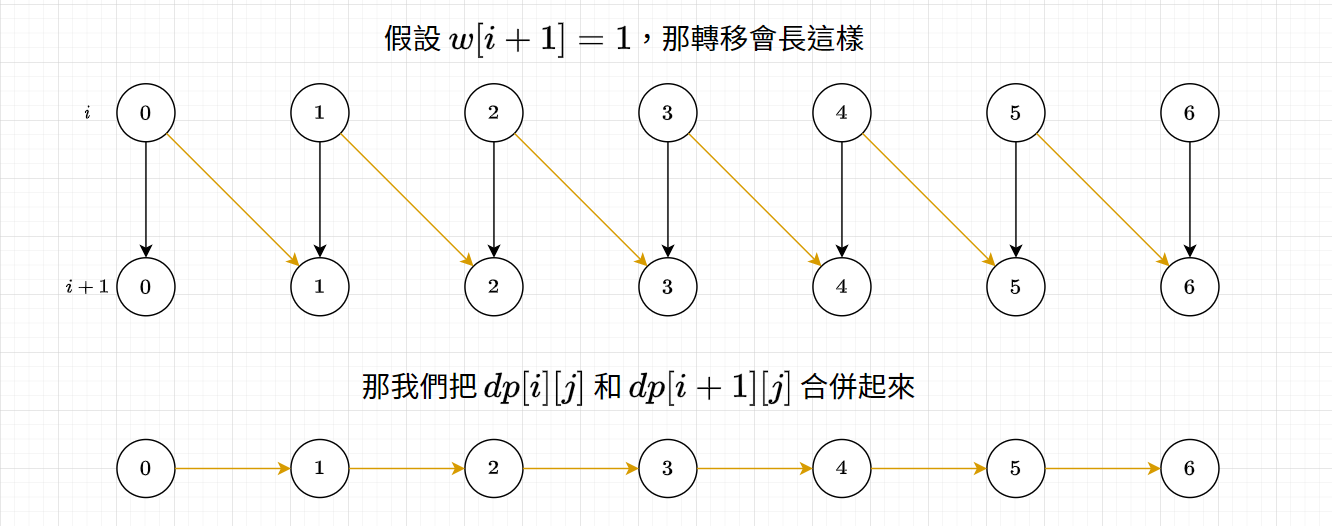
\includegraphics[scale=0.4]{images/rolling_01_knapsack.png}
        \end{center}
    \end{frame}
    
    \begin{frame}{背包問題 - 0}
        \begin{center}
            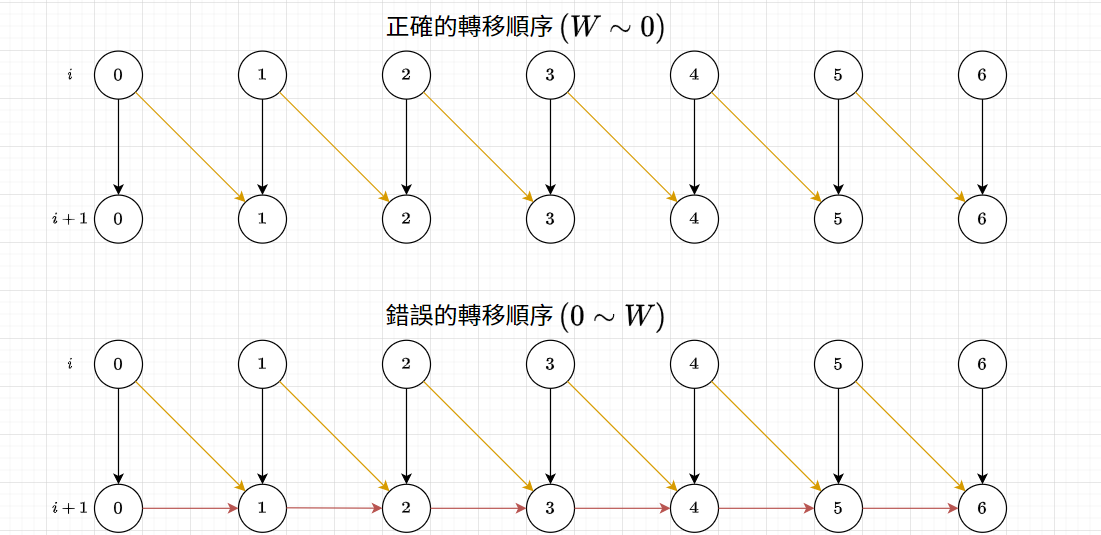
\includegraphics[scale=0.4]{images/rolling_01_knapsack_transition.png}
        \end{center}
    \end{frame}
    
    \begin{frame}[fragile]{背包問題 - 0}
        \begin{lstlisting}[language=C++, basicstyle=\ttfamily\tiny]
#include <bits/stdc++.h>
#define fastio ios_base::sync_with_stdio(false);cin.tie(0);

using namespace std;

signed main(){
    fastio

    int N,W;cin>>N>>W;
    int w[N+1]{},v[N+1]{};
    for(int i=1;i<=N;++i) cin>>w[i]>>v[i];
    long long dp[W+1]{};
    for(int i=1;i<=N;++i){
        for(int j=W;j>=0;--j){
            if(j>=w[i]) dp[j]=max(dp[j],dp[j-w[i]]+v[i]);
        }
    }
    cout<<dp[W]<<'\n';
}
        \end{lstlisting}
\end{frame}

    \begin{frame}{背包問題 - 1}
        \begin{block}{無限背包問題}
            有 $N$ 個物品,每個物品有價值 $v_i$ 和大小 $w_i$,每種物品有無限多個。你有一個容量為 $W$ 的背包。請問你最多可以拿多少價值?
        \end{block}
        \begin{itemize}
            \item<2-> 有注意到這題跟上一題不同的地方嗎?
            \item<3-> 他每個物品可以拿\textbf{無限}個!
        \end{itemize}
    \end{frame}

    \begin{frame}{背包問題 - 1}
        \begin{itemize}
            \item 其實只有轉移的地方需要修改
            \item<2-> 一樣是分選或不選,只是同個物品可以選了再選
        \end{itemize}
        $$
        dp[i][j]= \max
        \begin{cases}
            dp[i][j-w[i]]+v[i] & \text{選物品} \\
            dp[i-1][j]           & \text{不選物品} \\
        \end{cases}
        $$
    \end{frame}
    
    \begin{frame}[fragile]{背包問題 - 1}
    \begin{lstlisting}[language=C++,basicstyle=\ttfamily \tiny]
#include <bits/stdc++.h>
#define fastio ios_base::sync_with_stdio(false);cin.tie(0);
using namespace std;

signed main(){
    fastio

    int n,W;cin>>n>>W;
    int v[n+1]{},w[n+1]{};
    for(int i=1;i<=n;i++) cin>> v[i] >> w[i];

    int dp[n+1][W+1]{};
    for(int i=1;i<=n;i++){
        for(int j=1;j<=W;j++){
            dp[i][j]=dp[i-1][j];
            if(j-v[i]>=0) dp[i][j]=max(dp[i][j],dp[i][j-v[i]]+w[i]);
        }
    }
    int ans=0;
    for(int j=0;j<=W;j++) ans=max(dp[n][j],ans);

    cout<<ans<<'\n';
}
    \end{lstlisting}
    \end{frame}
    
    \begin{frame}{背包問題 - 2}
        \begin{block}{\href{https://cses.fi/problemset/task/1159}{CSES - Book Shop II}}
            有 $N$ 個物品,每個物品有價值 $v_i$ 和大小 $w_i$,每種物品有 $a_i$ 個。你有一個容量為 $W$ 的背包。請問你最多可以拿多少價值?
        \end{block}
        \begin{itemize}
            \item 這個是有限背包問題
        \end{itemize}
    \end{frame}
    
    \begin{frame}{背包問題 - 2}
        \begin{itemize}
            \item 如果能理解前面兩個問題,應該不難列出這個轉移式
            $$
            dp[i][j]= \max
            \begin{cases}
                dp[i][j-k*w[i]]+k*v[i] & \text{選 k 個物品} \\
                dp[i-1][j]           & \text{不選物品} \\
            \end{cases}
            $$
            \item 他的時間複雜度為 $O(NW\sum a_i)$
        \end{itemize}
    \end{frame}
    
    \begin{frame}[fragile]{背包問題 - 2}
        \begin{lstlisting}[language=C++,basicstyle=\ttfamily\tiny]
#include <bits/stdc++.h>
#define fastio ios_base::sync_with_stdio(false);cin.tie(0);
using namespace std;

signed main(){
    fastio

    int n,x;cin>>n>>x;
    int h[n+1]{},s[n+1]{},k[n+1]{};
    for(int i=1;i<=n;i++) cin>>h[i];
    for(int i=1;i<=n;i++) cin>>s[i];
    for(int i=1;i<=n;i++) cin>>k[i];

    int dp[n+1][x+1]{};
    for(int i=1;i<=n;i++){
        for(int j=1;j<=x;j++){
            dp[i][j]=dp[i-1][j];
            for(int kk=1;kk<=k[i];kk++){
                if(j-kk*h[i]>=0) dp[i][j]=max(dp[i][j],dp[i-1][j-kk*h[i]]+kk*s[i]);
            }
        }
    }
    int ans=0;
    for(int j=0;j<=x;j++) ans=max(dp[n][j],ans);

    cout<<ans<<'\n';
}
        \end{lstlisting}
    \end{frame}

    \begin{frame}{背包問題 - 2}
        \begin{itemize}
            \item 原本的作法,會去枚舉拿 $0,1,...,a_i$ 個物品,但是真的需要枚舉那麼多個嗎?
            \item<2-> 有甚麼辦法可以不用枚舉這麼多卻可以湊出 $0 \sim a_i$ 的每個數字?
            \item<3-> 想想看二進位!
            \item<4-> 這樣我們只需要枚舉 $\log a_i$ 個物品,而且有辦法湊出所有的數!
            \item<5-> 有人會叫這個東西叫二的冪次綑綁優化
            \item<6-> $O(NW \log \max(a_i))$
        \end{itemize}
    \end{frame}

    \section{其他練習題}
    
    \begin{frame}{練習題 - 0}
        \begin{block}{\href{https://codeforces.com/contest/1633/problem/D}{CodeForces D. Make Them Equal}}
            有一個陣列$a$,一開始所有數字都是$1$\\
            \vspace{2mm}
            每次操作可以選擇$i$和$x$,並且把$a[i] := a[i] + \Big \lfloor \dfrac{a_i}{x} \Big \rfloor$ \\
            \vspace{2mm}
            當$a[i]=b[i]$時,可以獲得$c_i$的錢,問在$k$次操作內,最多可以拿到多少錢?
            \vspace{2mm}
            \begin{itemize}
                \item $1\leq n\leq 10^3$
                \item $0\leq k\leq 10^6$
                \item $1\leq b_i\leq 10^3$
            \end{itemize}
        \end{block}
    \end{frame}

    \begin{frame}{練習題 - 0}
        \begin{itemize}
            \item 如果知道要把 $1$ 變成 $b_i$ 最少需要 $d_i$ 次操作
            \item<2-> 那我們可以把$c_i$當作物品的價值,$d_i$當作物品的大小,$k$為背包的容量
            \item<3-> 這樣不就變成背包問題了嗎!
            \item<4-> 那我們要怎麼知道$d_i$?
            \item<5-> 預處理就好了
        \end{itemize}
    \end{frame}

    \begin{frame}{練習題 - 0}
        \begin{itemize}
            \item 這樣做的時間複雜度為 $O(nk)$
            \item 可是這樣不會 TLE 嗎?
            \item 其實不會,但如果把 $d_i$ 全部輸出看看,會發現 $d_i$ 不會超過 $12$
            \item 所以其實可以只跑到 $12n$,因此複雜度其實只需要 $O(12n^2)$
        \end{itemize}
    \end{frame}

    \begin{frame}[fragile]{練習題 - 0}
        \begin{lstlisting}[language=C++,basicstyle=\ttfamily\tiny]
int n,k,r,a[MAXN],b[MAXN],c[MAXN];
void init(){
    for(int i=2;i<MAXN;++i) a[i]=MAXN;
    a[1]=0,r=0;
    for(int i=1;i<MAXN;++i){
        for(int j=1;j<=i;++j) if(i+i/j<MAXN) a[i+i/j]=min(a[i]+1,a[i+i/j]);
    }
}
void solve(){
    cin>>n>>k;
    init();
    for(int i=1;i<=n;++i) cin>>b[i];
    for(int i=1;i<=n;++i) cin>>c[i];   
    for(int i=1;i<=n;++i) r+=a[b[i]];
    k=min(k,r);
    int dp[k+1]{};
    for(int i=1;i<=n;++i){
        for(int j=k;j>=0;--j){
            if(j>=a[b[i]]) dp[j]=max(dp[j],dp[j-a[b[i]]]+c[i]);
        }
    }
    cout<<*max_element(dp,dp+k+1)<<'\n';
}
signed main(){
    int T;cin>>T;
    while(T--){
        solve();
    }
}       
        \end{lstlisting}
    \end{frame}

    \begin{frame}{練習題 - 0}
        \begin{itemize}
            \item 會出現在比賽中的題目基本上是不會出現裸背包問題的
            \item 通常會像這題一樣經過包裝 ><
        \end{itemize}
    \end{frame}

    \begin{frame}{練習題 - 1}
        \begin{block}{\href{https://atcoder.jp/contests/abc134/tasks/abc134_e}{Atcoder E - Sequence Decomposing}}
            給你一個陣列 $a$,問你最少可以將這個陣列分成幾個遞增子序列
        \end{block}
    \end{frame}

    \begin{frame}{練習題 - 1}
        \begin{itemize}
            \item 考慮貪心,維護多個遞增的子序列
        \end{itemize}
        \begin{center}
            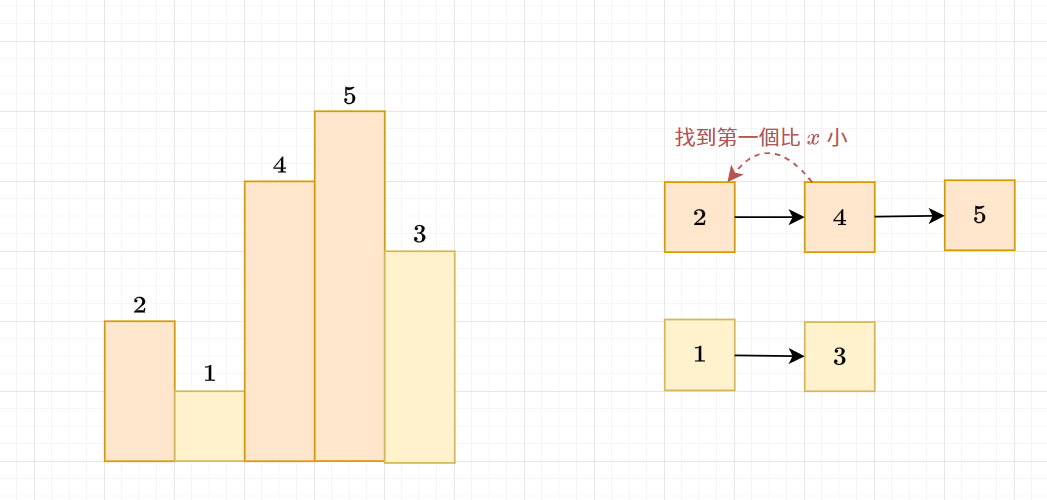
\includegraphics[scale=0.25]{images/ABC134E_Greedy.png}
        \end{center}
    \end{frame}
    
    \begin{frame}{練習題 - 1}
        \begin{itemize}
            \item 發現這樣做,其實等價於 LDS (Longest Decreasing Sequence)
        \end{itemize}
        \begin{center}
            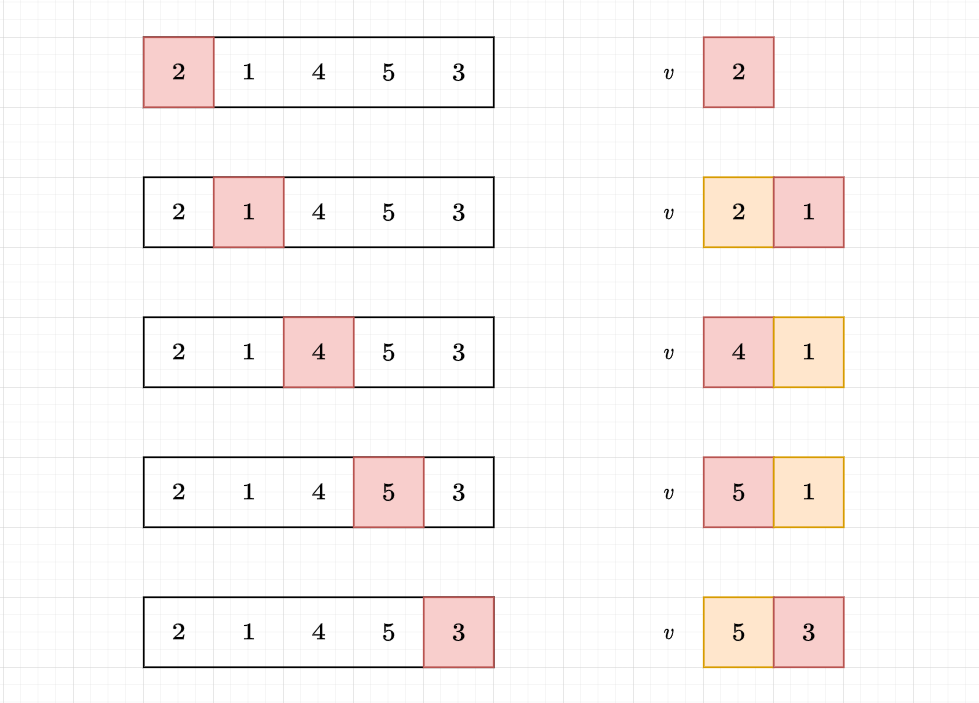
\includegraphics[scale=0.25]{images/ABC134E_LDS.png}
        \end{center}
    \end{frame}

    \begin{frame}[fragile]{練習題 - 1}
        \begin{lstlisting}[language=C++, basicstyle=\ttfamily\tiny]
#include <bits/stdc++.h>
#define fastio ios_base::sync_with_stdio(false);cin.tie(0);

using namespace std;

signed main(){
    fastio

    int n;cin>>n;
    int v[n+1]{};
    vector<int> lis;
    for(int i=n;i>=1;--i) cin>>v[i];
    for(int i=1;i<=n;++i){
        int now=upper_bound(lis.begin(),lis.end(),v[i])-lis.begin();
        if(now==lis.size()) lis.emplace_back(v[i]);
        else lis[now]=v[i];
    }
    cout<<lis.size()<<'\n';
}
        \end{lstlisting}
    \end{frame}

    \begin{frame}{練習題 - 2}
        \begin{block}{\href{https://tioj.ck.tp.edu.tw/problems/2048}{TIOJ 2048 - 最大不連續和問題}}
            給你一個 $N$ 項的陣列 $a$,請找到不連續的子序列中最大的總和是多少?
            \begin{itemize}
                \item $3 \le N \le 10^6$
                \item $|a_i| \le 10^9$
            \end{itemize}
        \end{block}
    \end{frame}

     \begin{frame}{練習題 - 2}
        \begin{itemize}
           \item 一樣按照之前的 dp 三步驟去想想看
           \item 先設好狀態!
        \end{itemize}
     \end{frame}

     \begin{frame}{練習題 - 2}
         \begin{alertblock}{step 1 設置狀態}
            我們可以把狀態設成以下這樣:
            \begin{align*}
                dp[0][j] &= \text{前} \ j \text{ 項的最大不連續和} \\
                dp[1][j] &= \text{前} \ j \text{ 項的最大連續和}   \\
                dp[2][j] &= \text{前} \ j \text{ 項不選} \ j       \\
            \end{align*}
            那麼答案就會是 $dp[0][N]$
        \end{alertblock}
     \end{frame}

     \begin{frame}{練習題 - 2}
        \setbeamercolor{block title}{use=structure,bg=green!50!black}
        \begin{block}{step 2 導出轉移}
            \begin{align*}
                dp[0][i] &= \max(dp[0][i-1]+\max(0,a[i]),dp[2][i-1]+a[i]) \\
                dp[1][i] &= \max(dp[1][i-1]+a[i],a[i])                   \\
                dp[2][i] &= \max(dp[2][i-1],dp[1][i-1])                  \\
            \end{align*} 
        \end{block}
    \end{frame}  
    
    \begin{frame}{練習題 - 2}
        \setbeamercolor{block title}{use=structure,bg=blue!60!black}
        \begin{block}{step 3 打好基底}
            因為 $a_i$ 有可能是負的,所以初始化的時候要設為 $-\infty$
        \end{block}
    \end{frame}
    
    \begin{frame}[fragile]{練習題 - 2}
        \begin{lstlisting}[language=C++, basicstyle=\ttfamily \tiny]
int dp[3][1000005]{},a[1000005]{};

void solve(){
    int n;cin>>n;
    for(int i=1;i<=n;++i) cin>>a[i];
    dp[0][0]=-1e18,dp[1][0]=-1e18,dp[2][0]=-1e18;
    for(int i=1;i<=n;++i){
        dp[0][i]=max(dp[0][i-1]+max(0LL,a[i]),dp[2][i-1]+a[i]);
        dp[1][i]=max(dp[1][i-1]+a[i],a[i]);
        dp[2][i]=max(dp[2][i-1],dp[1][i-1]);
    }
    cout<<dp[0][n]<<'\n';
}
        \end{lstlisting}
    \end{frame}

    \begin{frame}{練習題 - 3}
        \begin{block}{\href{https://codeforces.com/contest/1393/problem/D}{Codeforces 1393D Rarity and New Dress}}
            給你一個 $n \times m$ 的網格,每個格子上寫著一個字母,你要計算在這裡面有幾個轉了 $45^{\circ}$ 的正方形。
            \begin{itemize} 
                \item $1 \le n,m \le 2000$
            \end{itemize}
        \end{block}
    \end{frame}

    \begin{frame}{練習題 - 3}
        \begin{itemize}
            \item 沒想法的話可以先來觀察一下這個圖形
        \end{itemize}
         \begin{center}
            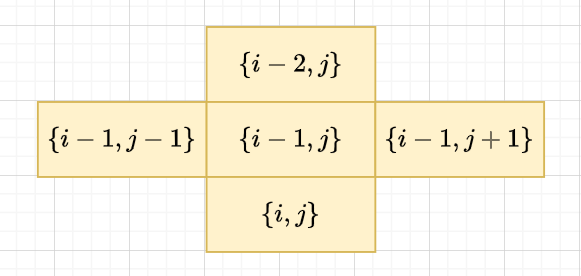
\includegraphics[scale=0.5]{images/CF1393D_i,j.png}
        \end{center}
        \begin{itemize}
            \item<2-> 很顯然的,如果要構成一個邊長為 $2$ 的正方形,則必須符合
            $$f_{i,j} = f_{i-1,j} = f_{i-2,j} = f_{i-1,j-1} = f_{i-1,j+1}$$
        \end{itemize}
    \end{frame}

    \begin{frame}{練習題 - 3}
        \begin{center}
            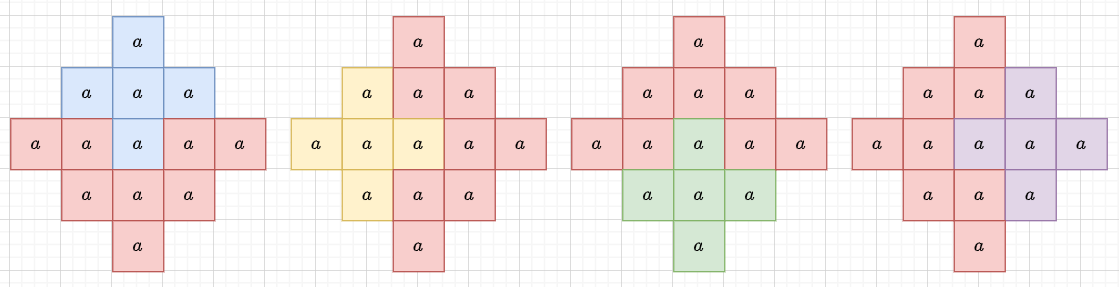
\includegraphics[scale=0.5]{images/CF1393D_square.png}
        \end{center}
        \begin{itemize}
            \item<2-> 由圖可知,邊長為 $3$ 的正方形是$4$個邊長為$2$的正方形組成的
            \item<3-> 同理,邊長為 $4$ 的正方形是$4$個邊長為$3$的正方形組成的
        \end{itemize}
    \end{frame}

    \begin{frame}{練習題 - 3}
        \begin{alertblock}{step 1 設置狀態}
            令$dp[i][j]$為當正方形右下角位於座標${i,j}$時的合法正方形數量\\
            \vspace{2mm}
            那麼答案就會是 $$\max_{i \le n,j \le m}dp[i][j]$$
        \end{alertblock}
    \end{frame}

    \begin{frame}{練習題 - 3}
        \setbeamercolor{block title}{use=structure,bg=green!50!black}
        \begin{block}{step 2 導出轉移}
            如果 $g[i][j]=g[i-1][j]=g[i-2][j]=g[i-1][j+1]=g[i-1][j-1]$,則轉移式為
            $$dp[i][j] \coloneqq \min\{dp[i-2][j],dp[i-1][j-1],dp[i-1][j+1]\} + 1$$
            表示我們可以用小的正方形去組成大的正方形
        \end{block}
    \end{frame}
    
    \begin{frame}{練習題 - 3}
        \begin{block}{step 3 打好基底}
            每一格自己都是一個合法的正方形\\
            $$dp[i][j]=1$$
        \end{block}
    \end{frame}

    \begin{frame}[fragile]{練習題 - 3}
        \begin{lstlisting}[language=C++, basicstyle=\ttfamily\tiny]
#include <bits/stdc++.h>
#define fastio ios_base::sync_with_stdio(false);cin.tie(0);

using namespace std;

char g[2005][2005];
vector<vector<int>> dp(2005,vector<int>(2005,1));

signed main(){
    fastio

    int n,m;cin>>n>>m;
    for(int i=1;i<=n;++i){
        for(int j=1;j<=m;++j) cin>>g[i][j];
    }
    int ans=0;
    for(int i=1;i<=n;++i){
        for(int j=1;j<=m;++j){
            if(g[i][j]==g[i-1][j]&&g[i][j]==g[i-2][j]&&g[i][j]==g[i-1][j+1]&&g[i][j]==g[i-1][j-1]){
                dp[i][j]+=min({dp[i-1][j-1],dp[i-1][j+1],dp[i-2][j]});
            }
            ans+=dp[i][j];
        }
    }
    cout<<ans<<'\n';
}
        \end{lstlisting}
    \end{frame}

    \begin{frame}{練習題 - 3}
        \begin{itemize}
            \item 官解有提供另外一種方法
            \item 實作比較麻煩一點
            \item 但可能比較好想(?
            \item 有興趣的可以去看看
            \item \href{https://codeforces.com/blog/entry/81161}{1393D - Rarity and New Dress solution}
        \end{itemize}
    \end{frame}

    \begin{frame}{練習題 - 4}
        \begin{block}{\href{https://tioj.ck.tp.edu.tw/problems/2173}{2019 北市賽 - 搜集寶藏 (Treasure)}}
            給你一個$M\times N$的網格圖上面有很多寶藏,有兩個人要從左上角走去右下角,而且只能往右或往下移動,寶藏不可重複領取,問最多能拿到幾個寶藏
            \begin{itemize}
                \item $2\leq M,N \leq 100$
            \end{itemize}
        \end{block}
    \end{frame}

    \begin{frame}{練習題 - 4}
        \begin{itemize}
            \item 如果先讓一個人走完再讓另一個人走
            \item 兩個人都用最佳策略去走,會是最佳解嗎?
            \begin{center}
                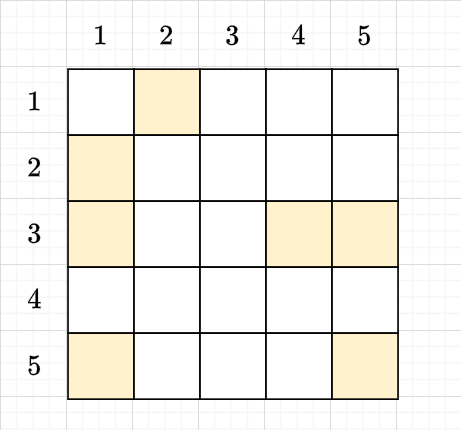
\includegraphics[scale=0.5]{images/treasure_counterexample.png}
            \end{center}
            \item<2-> \textcolor{red}{WA!}
        \end{itemize}
    \end{frame}

    \begin{frame}{練習題 - 4}
        \begin{itemize}
            \item 這樣看來分開做是不行的,我們需要同時維護兩個人一起移動的答案
            \item<2-> 設置狀態: $dp[x_1][y_1][x_2][y_2]$ 表示兩人分別走到 $(x_1,y_1), \ (x_2,y_2)$ 的答案
            \item<3-> 這樣會 \textcolor{yellow}{MLE}
        \end{itemize}
    \end{frame}

    \begin{frame}{練習題 - 4}
        \begin{itemize}
            \item 要怎麼減少狀態?
            \item<2-> 你會發現在第 $k$ 分鐘時,$x_1+y_1=x_2+y_2=k$
            \item<3-> 減少狀態:$dp[k][x_1][x_2]$
            \item<4-> 雖然沒必要,但想要壓常的話可以滾動
            \item<5-> 小提醒:這題的轉移式跟之前的格子路徑差不多,但是要注意兩個人走到同一個位置的時候,不能重複計算
        \end{itemize}
    \end{frame}
    
\end{document}